\documentclass{article}
\usepackage[utf8]{inputenc}
\usepackage[
  colorlinks=true,
  linkcolor=blue,
  filecolor=blue,
  urlcolor=blue,
]{hyperref}
\usepackage{graphicx}
\usepackage[rightcaption]{sidecap}


\graphicspath{ {./assets/} }

\newcommand{\gh}[1]{%
  \href{https://github.com/awave1/cpsc501-tensorflow/commit/#1}{#1}%
}


\title{CPSC 501 -- Assignment 4}
\author{Artem Golovin \\ 30018900}
\date{December 2019}

\begin{document}

\maketitle

\section*{Part 1}

To optimize the given MNIST model, I performed the following:

\begin{itemize}
  \item Added a Dense layer with 512 neurons
  \item To prevent overfitting, Dropout layer was added as well
  \item The algorithm was changed to `Adam'
  \item Number of epochs increased from 1 to 10
\end{itemize}

Resulting model is 99\% accurate on the training data and 98\% accurate on the test data.

\subsubsection*{References}

\begin{itemize}
  \item \href{https://www.tensorflow.org/tutorials/quickstart/beginner}{https://www.tensorflow.org/tutorials/quickstart/beginner}
\end{itemize}

\section*{Part 2}

\subsection*{Part 2.1}

Initial model for Part 2 was using the same layers as the model for Part 1, which can be seen here \gh{14cec7c3}. The accuracy with that model was roughly 93\%. However, the model failed to identify image \texttt{user\_inputs/image\_A\_lower.png}.

\subsection*{Part 2.2}

To improve the model, I implemented a Convolution Neural Network, which increased the accuracy of notMNIST model to roughly 95\%. This model was able to identify the image \texttt{user\_inputs/image\_A\_lower.png}.

Besides the convolution network, adding more neurons via extra Dense layers and Dropout layers that prevent overfitting increased the predictions.

\begin{figure}[t]
  \caption{Initial test with the first model}
  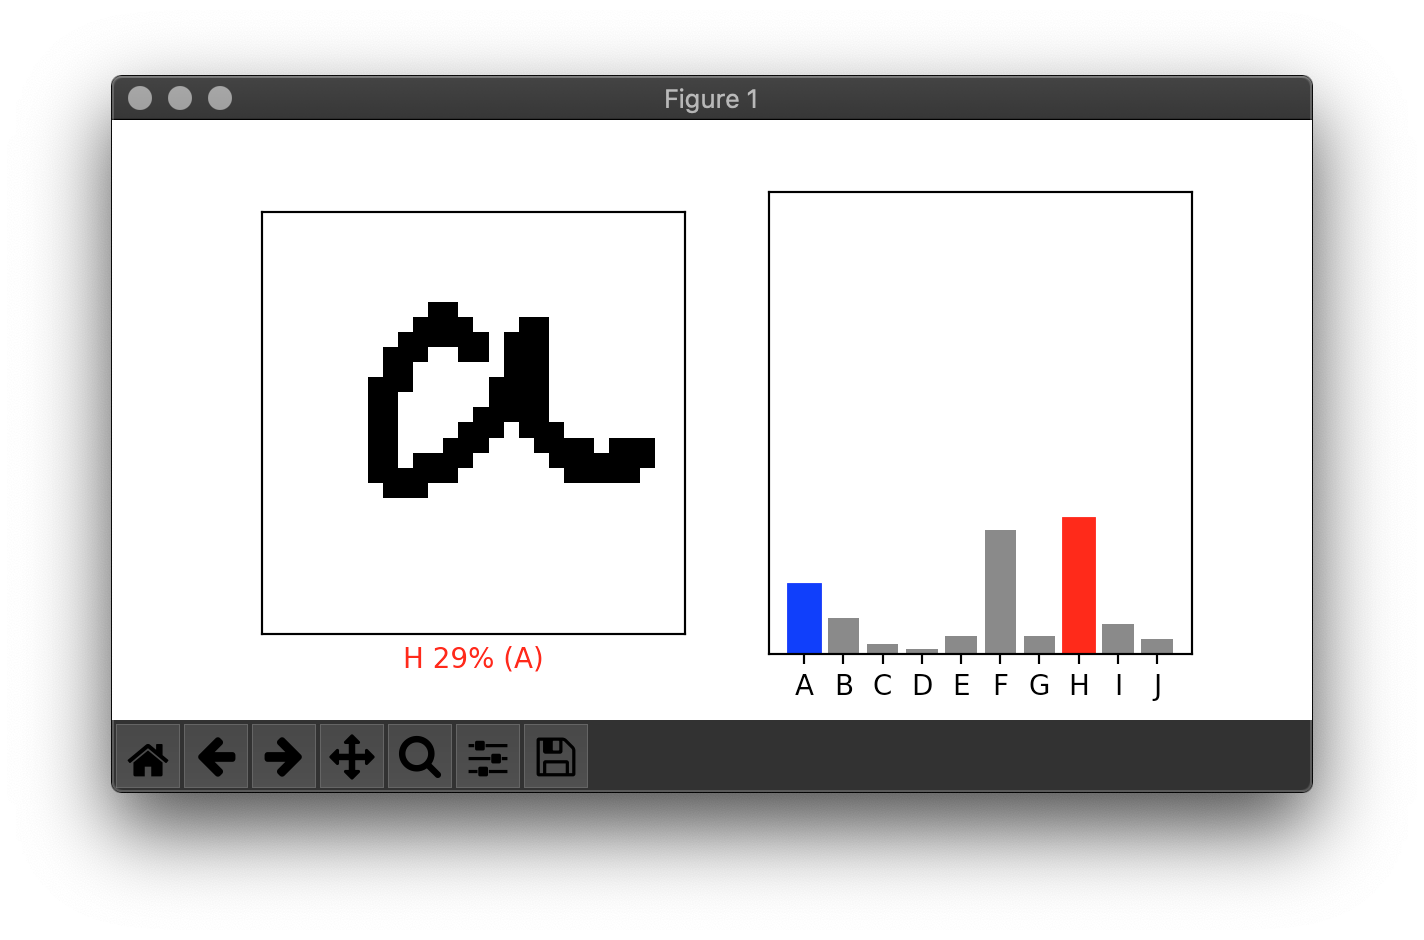
\includegraphics[width=0.6\textwidth]{user_input_a}
  \centering
  \caption{Test using the updated model}
  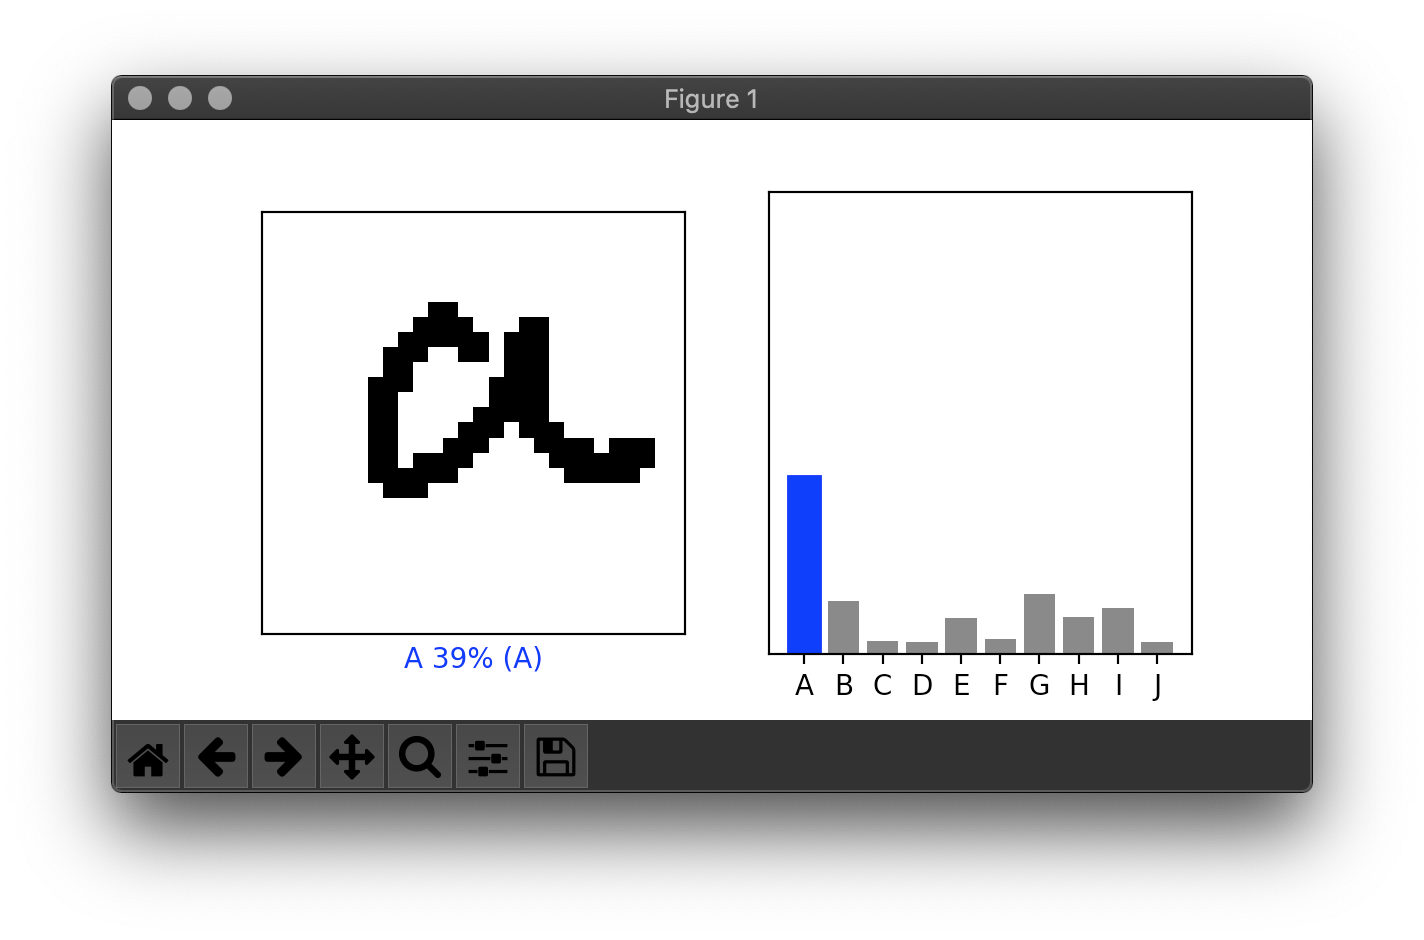
\includegraphics[width=0.6\textwidth]{user_input_b}
  \centering
\end{figure}

\section*{Part 3}

Initially, the model was trained without taking in consideration overfitting. Resulted accuracy:

\begin{figure}[h!]
  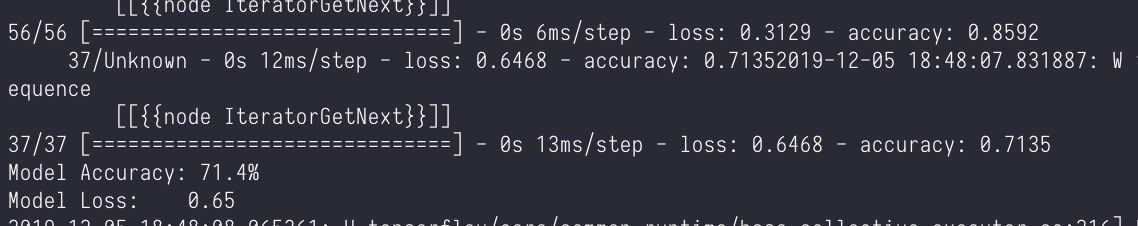
\includegraphics[width=0.8\textwidth]{p32.png}
  \centering
\end{figure}

After adding Dropouts and l2 regularizers, the model testing and training accuracy align and become roughly equal:

\begin{figure}[h!]
  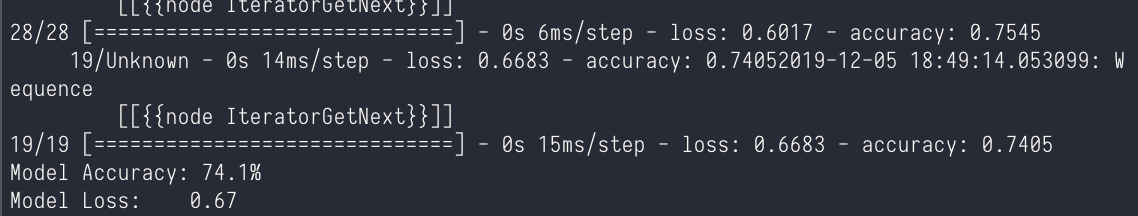
\includegraphics[width=0.8\textwidth]{p31.png}
  \centering
\end{figure}

\newpage

\subsubsection*{References}

\begin{itemize}
  \item \href{https://www.tensorflow.org/tutorials/load\_data/csv}{https://www.tensorflow.org/tutorials/load\_data/csv}
  \item \href{https://www.tensorflow.org/tutorials/keras/overfit\_and\_underfit}{https://www.tensorflow.org/tutorials/keras/overfit\_and\_underfit}
\end{itemize}

\end{document}